\subsection{Instance models}
\label{subsec:formalisations:ecore_formalisation:instance_models}
An instance model represents an instance of a type model. In other words, the metamodel of an instance model is its type model. Because of our definitions of type models, this means that the metametamodel of an instance model is the Ecore metamodel.

An instance model consists of a set of objects, which have a corresponding class they instantiate and an optional identifier. All objects are an instance of a specific class and are therefore typed by that class and its superclasses. Furthermore, an instance model also specifies the values for each field of an object. Its type determines the fields present for each object. Finally, the instance model specifies a set of default values, which assigns a value to each of the named constants from the type model ($Constant_{Tm}$), allowing to assign default values to fields.

As with the type model and type definitions, there is a cyclic dependency between instance models and values. In the same manner, the solution is set to be the smallest solution to the set of equations for the instance model and values.

The suffix $Im$ is used when the definition of something depends on any instance model $Im$, which itself depends on the definition of any type model $Tm$.

\begin{defin}[Instance model]
\label{defin:formalisations:ecore_formalisation:instance_models:instance_model}
For a type model $Tm$,
\begin{equation*}
    Tm = \langle Class, Enum, UserDataType, Field, \mathrm{FieldSig}, EnumValue, Inh, Prop, Constant, \mathrm{ConstType} \rangle
\end{equation*}
a single instance model $Im$ is defined as
\begin{equation*}
    Im = \langle Object, \mathrm{ObjectClass}, \mathrm{ObjectId}, \mathrm{FieldValue}, \mathrm{DefaultValue} \rangle
\end{equation*}
with
\begin{itemize}
    \item $Object$ is the set of objects (class instances) in $Im$.
    \item $\mathrm{ObjectClass}: Object \Rightarrow Class_{Tm}$ is the function that maps each object in $Im$ to a class.
    \item $\mathrm{ObjectId}: Object \Rightarrow Name$ is the injective partial function that maps each object in $Im$ to an identifier.
    \item $\mathrm{FieldValue}: (Object \times Field_{Tm}) \Rightarrow Value_{Im}$ is the partial function between each $Field_{Tm}$ of an $Object_{Im}$ and a $Value_{Im}$ (see \cref{defin:formalisations:ecore_formalisation:instance_models:values}).
    \item $\mathrm{DefaultValue}: Constant_{Tm} \Rightarrow Value_{Im}$ is the function that assigns a value to each constant in the corresponding type model $Tm$.
\end{itemize}
where
\begin{itemize}
    \item $\forall ( o, n ), ( o', n' ) \in ObjectId: n = n' \Longrightarrow o = o'$.
    \item $\forall o \in Object, f \in Field_{Tm}: ( o, f ) \in \mathrm{dom}\ FieldValue \Longleftrightarrow ObjectClass(o) \sqsubseteq_{Tm} \mathrm{class}(f)$.
\end{itemize}

\isabellelref{instance_model}{Ecore.Instance_Model}
\end{defin}

Please note that $\mathrm{ObjectId}$ is injective because each object must have a unique identifier. It is partial because an object does not necessarily need an identifier: The internal object identifiers (the elements of the set $Object$) are already unique. The $\mathrm{ObjectId}$ function is for adding an explicit identifier that is not generated internally.

The $\mathrm{FieldValue}$ function maps a combination of an object and field to a value. Please note that the function is partial because not every combination of object and field is valid. The domain of this function is therefore made explicit by the constraints of the definition. Please note that this function is not injective: Values can be shared across objects and do not have to be unique.

An important function is the $\mathrm{DefaultValue}$ function, which is defined on an instance model rather than a type model. This definition has been chosen to accommodate for default values that reference another object. In order to reference another object, the possible object references need to be known. These object references are only known on the instance level, as the type level does not define any objects.

\begin{figure}[p]
    \centering
    \begin{subfigure}{\textwidth}
        \centering
        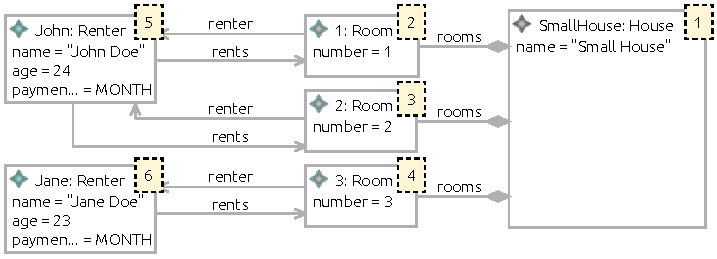
\includegraphics{images/03_formalisations/02_ecore_formalisation/instance_model_example.pdf}
        \caption{Instance model based on Ecore notation}
    \end{subfigure}
    
    \begin{subfigure}{\textwidth}
        \centering
        \begin{align*}
            Object_{Im} =\ & \{ 
                1, 2, 3, 4, 5, 6
            \}\\
            \mathrm{ObjectClass}_{Im} =\ & \{ 
                ( 1, .\type{House} ),
                ( 2, .\type{Room} ),
                ( 3, .\type{Room} ), 
                ( 4, .\type{Room} ),
                ( 5, .\type{Renter} ),
                ( 6, .\type{Renter} ),
            \}\\
            \mathrm{ObjectId}_{Im} =\ & \{ 
                ( 1, .\type{SmallHouse} ),
                ( 2, .\type{1} ),
                ( 3, .\type{2} ), 
                ( 4, .\type{3} ),
                ( 5, .\type{John} ),
                ( 6, .\type{Jane} )
            \}\\
            \mathrm{FieldValue}_{Im} =\ & \Big\{ 
                \Big( \big( 1, ( .\type{House}, \type{name} ) \big), \big[ \type{string}, \text{``Small House''} \big] \Big),\\&
                \Big( \big( 1, ( .\type{House}, \type{rooms} ) \big), \big[ \type{setof}, \big\langle [ \type{obj}, 2 ], [ \type{obj}, 3 ], [ \type{obj}, 4 ] \big\rangle \big] \Big),\\&
                \Big( \big( 2, ( .\type{Room}, \type{number} ) \big), \big[ \type{int}, 1 \big] \Big),\
                \Big( \big( 2, ( .\type{Room}, \type{renter} ) \big), \big[ \type{obj}, 5 \big] \Big),\\&
                \Big( \big( 3, ( .\type{Room}, \type{number} ) \big), \big[ \type{int}, 2 \big] \Big),
                \Big( \big( 3, ( .\type{Room}, \type{renter} ) \big), \big[ \type{obj}, 5 \big] \Big),\\&
                \Big( \big( 4, ( .\type{Room}, \type{number} ) \big), \big[ \type{int}, 3 \big] \Big),
                \Big( \big( 4, ( .\type{Room}, \type{renter} ) \big), \big[ \type{obj}, 6 \big] \Big),\\&
                \Big( \big( 5, ( .\type{Person}, \type{name} ) \big), \big[ \type{string}, \text{``John Doe''} \big] \Big),\\&
                \Big( \big( 5, ( .\type{Person}, \type{age} ) \big), \big[ \type{int}, 24 \big] \Big),\\&
                \Big( \big( 5, ( .\type{Renter}, \type{payment\_interval} ) \big), \big[ \type{enum}, ( .\type{PaymentInterval}, \type{MONTH} ) \big] \Big),\\&
                \Big( \big( 5, ( .\type{Renter}, \type{rents} ) \big), \big[ \type{setof}, \big\langle [ \type{obj}, 2 ], [ \type{obj}, 3 ] \big\rangle \big] \Big),\\&
                \Big( \big( 6, ( .\type{Person}, \type{name} ) \big), \big[ \type{string}, \text{``Jane Doe''} \big] \Big),\\&
                \Big( \big( 6, ( .\type{Person}, \type{age} ) \big), \big[ \type{int}, 23 \big] \Big),\\&
                \Big( \big( 6, ( .\type{Renter}, \type{payment\_interval} ) \big), \big[ \type{enum}, ( .\type{PaymentInterval}, \type{MONTH} ) \big] \Big),\\&
                \Big( \big( 6, ( .\type{Renter}, \type{rents} ) \big), \big[ \type{setof}, \big\langle [ \type{obj}, 4 ] \big\rangle \big] \Big)
            \Big\}\\
            \mathrm{DefaultValue}_{Im} =\ & \Big\{ 
                \Big( .\type{Constant}.\type{PaymentInterval}.\type{Month}, \big[ \type{enum}, ( .\type{PaymentInterval}, \type{MONTH} ) \big] \Big)
            \Big\}
        \end{align*}
        \caption{Formal definition of the instance model}
    \end{subfigure}
    \caption{Example of an instance model corresponding with \cref{defin:formalisations:ecore_formalisation:instance_models:instance_model}}
    \label{fig:formalisations:ecore_formalisation:instance_models:instance_model_example}
\end{figure}

An example model is represented by \cref{fig:formalisations:ecore_formalisation:instance_models:instance_model_example}. It is based on the type model from the example in \cref{fig:formalisations:ecore_formalisation:type_models:type_model_example}.
It shows 2 instantiations of the $\type{Renter}$ class: the $\type{John}$ and $\type{Jane}$ objects. Furthermore, there are three instantiations of the $\type{Room}$ class ($\type{1}$, $\type{2}$ and $\type{3}$) and one instantiation of the $\type{House}$ class ($\type{SmallHouse}$). The text after the colon in the header of each object represents the $ObjectClass_{Im}$ of each object. Additionally, the text preceding the colon represents the $ObjectId_{Im}$. The $\type{Renter}$ objects have values assigned for all fields, including the fields of their superclasses. This also holds for the $\type{Room}$ and $\type{House}$ objects. For attributes, the assignment to a field name represents the value of a field. For relations, a named arrow between two objects represents the value of the field. The name of the arrow represents the field name, and multiple arrows with the same name represent multiple values for the same field.

Note that the objects from the example are represented by elements from $\mathbb{N}^+$. The conceptual model does not give a concrete specification for elements in the $Object_{Im}$ set, but by convention objects (or in graph terms, nodes) are represented by numbers.

For each instance model, a set of possible values is defined by the values for all data types, the possible enumerations of the type model and the objects in the instance model. Each value has a symbol that defines its type, allowing the values in an instance model to be typed by the types in the type model. This symbol also allows values with identical content but a different type to be separated. For example, any value in $\mathbb{Z} \cap \mathbb{R}$ (which can be of type $\type{integer}$ or $\type{real}$). Container values aggregate multiple values, which are typed by container types.

\begin{defin}[Values]
\label{defin:formalisations:ecore_formalisation:instance_models:values}
Given any instance model $Im$, the set of values is $Value_{Im}$.

The set of values is then defined as
\begin{equation*}
    Value_{Im} = AtomValue_{Im} \cup ContainerValue_{Im}
\end{equation*}
with
\begin{itemize}
    \item $AtomValue_{Im} = ClassValue_{Im} \cup LiteralValue \cup (\{ \type{enum} \} \times EnumValue_{Tm}) \cup (\{ \type{data} \times \mathbb{S}\})$
    \item $LiteralValue = (\{ \type{bool} \} \times \mathbb{B}) \cup (\{ \type{int} \} \times \mathbb{Z}) \cup (\{ \type{real} \} \times \mathbb{R}) \cup (\{ \type{string} \} \times \mathbb{S})$
    \item $ClassValue_{Im} = \{ \type{obj} \} \times (Object_{Im} \cup { \type{nil} })$
    \item $ContainerValue_{Im} = \{ \type{setof}, \type{bagof}, \type{seqof}, \type{ordof} \} \times Value_{Im}^*$ (where $Value_{Im}^*$ allows containers to recursively contain other containers.)
\end{itemize}

The set of values is recursively defined as the smallest solution of the given set of equations for $Value_{Im}$ and $ContainerValue_{Im}$. Furthermore, elements of the set $Value_{Im}$ are written using square brackets, e.g. $[\type{string}, \text{``Example''}]$ or $[\type{setof}, \langle [\type{int}, 4], [\type{int}, 8] \rangle]$.

\isabellelref{Value}{Ecore.Instance_Model}
\end{defin}

For custom data types, the value is an element from the set $\mathbb{S}$. In Ecore, custom data types can be made serializable, which means a value from $\mathbb{S}$ can be stored for the custom data type. Thus, the value for a custom data type can be stored in the model, but it cannot be further interpreted.

Containers attributed as $\type{setof}$ or $\type{ordof}$ are considered to have unique values, whereas containers attributed as $\type{bagof}$ or $\type{seqof}$ are not. This means for example that a tuple with two or more identical values is not a valid value for a container attributed as $\type{setof}$ or $\type{ordof}$, see also \cref{defin:formalisations:ecore_formalisation:instance_models:valid_type_values}.

Additionally, the values of a container attributed as $\type{bagof}$ or $\type{setof}$ are considered unordered, and $\type{seqof}$ or $\type{ordof}$ ordered. This affects the equivalency of containers, as defined in \cref{defin:formalisations:ecore_formalisation:instance_models:value_equivalency}.

In the example, the set of atomic values that are assigned consists of
\begin{align*}
    \{&
        [ \type{string}, \text{``Small House''} ], 
        [ \type{string}, \text{``John Doe''} ], 
        [ \type{string}, \text{``Jane Doe''} ],\\&
        [ \type{int}, 1 ], 
        [ \type{int}, 2 ], 
        [ \type{int}, 3 ], 
        [ \type{int}, 24 ], 
        [ \type{int}, 23 ],\\&
        [ \type{enum}, ( .\type{PaymentInterval}, \type{MONTH} ) ]\\&
        [ \type{obj}, 5 ],
        [ \type{obj}, 6 ]
    \}
\end{align*}
Note that only the $\type{Renter}$ objects are in an atomic assigned value for the field $(.\type{Room}, \type{renter})$, as it is the only field that references a single object. All other relations in the type model are container types, and as such all the objects are contained in a container value as well. For example, the container value for the $\type{rooms}$ field of the $\type{House}$ object is $\big[ \type{setof}, \big\langle [ \type{obj}, 2 ], [ \type{obj}, 3 ], [ \type{obj}, 4 ] \big\rangle \big]$ (in no particular order, as the relation is of a set container type).

Each instance model also defines an equivalence relation for values. This relation allows the comparison of aggregate values and explicitly defines equivalency for unordered container values.

\begin{defin}[Value equivalency]
\label{defin:formalisations:ecore_formalisation:instance_models:value_equivalency}
Two values are equivalent $(\equiv_{Im}\: \subseteq Value_{Im} \times Value_{Im})$ if both the type is identical and the actual value content is equivalent. It is defined as the smallest reflexive relation between values and the relations defined by the rules given next.

For atomic values equivalence is defined as
\begin{mathpar}
    \inferrule{v_1 \in Value_{Im} \\ v_2 \in Value_{Im} \\ v_1 = v_2}{v_1 \equiv_{Im} v_2}
\end{mathpar}

Sequences and ordered sets are equivalent if the values in their tuples are pairwise equivalent.
\begin{mathpar}
    \inferrule[Sequence container equivalency]{c_1 = \big[ \type{seqof}, \langle v_1, \dotsc, v_n \rangle \big] \\ c_2 = \big[ \type{seqof}, \langle u_1, \dotsc, u_n \rangle \big] \\ v_1 \equiv_{Im} u_1, \dotsc, v_n \equiv_{Im} u_n}{c_1 \equiv_{Im} c_2}
\end{mathpar}
\begin{mathpar}
    \inferrule[Ordered set container equivalency]{c_1 = \big[ \type{ordof}, \langle v_1, \dotsc, v_n \rangle \big] \\ c_2 = \big[ \type{ordof}, \langle u_1, \dotsc, u_n \rangle \big] \\ v_1 \equiv_{Im} u_1, \dotsc, v_n \equiv_{Im} u_n}{c_1 \equiv_{Im} c_2}
\end{mathpar}

Sets and bags are equivalent if there exists a bijective function which maps elements from one set/bag
to the other, such that the mapped values are equivalent.
\begin{mathpar}
    \inferrule[Set container equivalency]{c_1 = \big[ \type{setof}, \langle v_1, \dotsc, v_n \rangle \big] \\ c_2 = \big[ \type{setof}, \langle u_1, \dotsc, u_n \rangle \big] \\ \exists f: \{1, \dotsc, n\} \bij \{1, \dotsc, n\}: v_i \equiv_{Im} u_{f(i)}}{c_1 \equiv_{Im} c_2}
\end{mathpar}
\begin{mathpar}
    \inferrule[Bag container equivalency]{c_1 = \big[ \type{bagof}, \langle v_1, \dotsc, v_n \rangle \big] \\ c_2 = \big[ \type{bagof}, \langle u_1, \dotsc, u_n \rangle \big] \\ \exists f: \{1, \dotsc, n\} \bij \{1, \dotsc, n\}: v_i \equiv_{Im} u_{f(i)}}{c_1 \equiv_{Im} c_2}
\end{mathpar}

\isabellelref{value_equiv}{Ecore.Instance_Model}
\end{defin}

In the example, the value $\big[ \type{setof}, \big\langle [ \type{obj}, 2 ], [ \type{obj}, 3 ] \big\rangle \big]$ would thus be equivalent to $\big[ \type{setof}, \big\langle [ \type{obj}, 3 ], [ \type{obj}, 2 ] \big\rangle \big]$, as the ordering does not matter for `$\type{setof}$' container types.

For each type in $Type_{Tm}$, there exists a set of values from $Value_{Im}$ which is considered \textit{valid}. This is
defined by a relation $Valid_{Im} \subseteq (Type_{Tm} \times Value_{Im})$ which defines a tuple for each valid value given a type.

\begin{defin}[Valid type values]
\label{defin:formalisations:ecore_formalisation:instance_models:valid_type_values}
The $Valid_{Im}$ set contains tuples which indicate what values are valid for a given type, which is defined by
\begin{equation*}
    Valid_{Im} \subseteq (Type_{Tm} \times Value_{Im})
\end{equation*}

An element $[ T, v ] \in Valid_{Im}$ may be written as
\begin{mathpar}
    \inferrule{\ }{v:_{Im} T}
\end{mathpar}

The contents of the $Valid_{Im}$ set is then defined as follows:

Data type values:
\begin{mathpar}
    \inferrule{v \in \mathbb{B}}{[ \type{bool}, v ]:_{Im} \type{boolean}}
    \and
    \inferrule{v \in \mathbb{Z}}{[ \type{int}, v ]:_{Im} \type{integer}}
    \and
    \inferrule{v \in \mathbb{R}}{[ \type{real}, v ]:_{Im} \type{real}}
    \and
    \inferrule{v \in \mathbb{S}}{[ \type{string}, v ]:_{Im} \type{string}}
\end{mathpar}

Class values:
\begin{mathpar}
    \inferrule{ObjectClass_{Im}(o) = c \\ !c \sqsubseteq_{Tm} t \\ t \in ClassType_{Tm}}{[ \type{obj}, o ]:_{Im} t}
    \and
    \inferrule{t \in \{ \type{nullable} \} \times Class_{Tm}}{[ \type{obj}, \type{nil} ]:_{Im} t}
\end{mathpar}

Enumeration values:
\begin{mathpar}
    \inferrule{( ename, eval ) \in EnumValue_{Tm} \\ ename \in Enum_{Tm}}{[ \type{enum}, ( ename, eval ) ]:_{Im} ename}
\end{mathpar}

User-defined data type values:
\begin{mathpar}
    \inferrule{v \in \mathbb{S} \\ t \in UserDataType_{Tm}}{[ \type{data}, v ]:_{Im} t}
\end{mathpar}

Container values:
\begin{mathpar}
    \inferrule{v_1:_{Im} T, \dotsc, v_n:_{Im} T \\ \langle v_1, \dotsc, v_n \rangle\ \mathrm{distinct} \\ [ \type{setof}, T ] \in Container_{Tm}}{[ \type{setof}, \langle v_1, \dotsc, v_n \rangle ]:_{Im} [ \type{setof}, T ]}
    \and
    \inferrule{v_1:_{Im} T, \dotsc, v_n:_{Im} T \\ [ \type{bagof}, T ] \in Container_{Tm}}{[ \type{bagof}, \langle v_1, \dotsc, v_n \rangle ]:_{Im} [ \type{bagof}, T ]}
    \and
    \inferrule{v_1:_{Im} T, \dotsc, v_n:_{Im} T \\ \langle v_1, \dotsc, v_n \rangle\ \mathrm{distinct} \\ [ \type{ordof}, T ] \in Container_{Tm}}{[ \type{ordof}, \langle v_1, \dotsc, v_n \rangle ]:_{Im} [ \type{ordof}, T ]}
    \and
    \inferrule{v_1:_{Im} T, \dotsc, v_n:_{Im} T \\ [ \type{seqof}, T ] \in Container_{Tm}}{[ \type{seqof}, \langle v_1, \dotsc, v_n \rangle ]:_{Im} [ \type{seqof}, T ]}
\end{mathpar}

\isabellelref{Valid}{Ecore.Instance_Model}
\end{defin}

The validity of an instance model depends on the multiplicity of field values. The valid multiplicities depend on the types and field signatures in the corresponding type model. As a consequence, a valid multiplicity also requires the type of the value to be valid. The multiplicity is of most influence for container values, as they can contain an arbitrary amount of values.

\begin{defin}[Multiplicity validity]
\label{defin:formalisations:ecore_formalisation:instance_models:multiplicity_validity}
A field value $( ( object, field ), value ) \in FieldValue_{Im}$ has a valid multiplicity if the following property holds:
\begin{multline*}
    value:_{Im} \mathrm{type}_{Tm}(field) \land value = [ t, \langle v_1, \dotsc, v_n \rangle ] \in ContainerValue_{Im} \Longrightarrow\\ \mathrm{lower}_{Im}(field) \leq n \leq \mathrm{upper}_{Im}(field)
\end{multline*}

This may be written as $\mathrm{validMul}_{Im}\big((( object, field ), value)\big)$.

\isabellelref{validMul}{Ecore.Instance_Model}
\end{defin}

\begin{figure}
    \centering
    \begin{subfigure}{\textwidth}
        \centering
        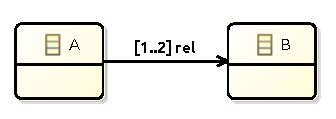
\includegraphics{images/03_formalisations/02_ecore_formalisation/multiplicities/type_model.pdf}
        \caption{Example type model}
        \label{fig:formalisations:ecore_formalisation:instance_models:multiplicity_example:type_model}
    \end{subfigure}
    
    \begin{subfigure}{0.3\textwidth}
        \centering
        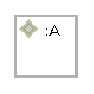
\includegraphics{images/03_formalisations/02_ecore_formalisation/multiplicities/invalid_lower.pdf}
        \caption{Invalid instance model: cardinality of $\type{rel}$ too low}
        \label{fig:formalisations:ecore_formalisation:instance_models:multiplicity_example:invalid_lower}
    \end{subfigure}
    \begin{subfigure}{0.3\textwidth}
        \centering
        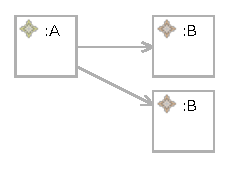
\includegraphics{images/03_formalisations/02_ecore_formalisation/multiplicities/valid.pdf}
        \caption{Valid instance model: cardinality of $\type{rel}$ within bounds}
        \label{fig:formalisations:ecore_formalisation:instance_models:multiplicity_example:valid}
    \end{subfigure}
    \begin{subfigure}{0.3\textwidth}
        \centering
        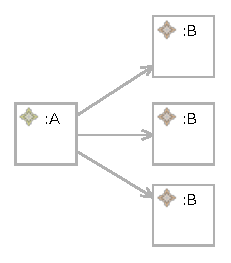
\includegraphics{images/03_formalisations/02_ecore_formalisation/multiplicities/invalid_upper.pdf}
        \caption{Invalid instance model: cardinality of $\type{rel}$ too high}
        \label{fig:formalisations:ecore_formalisation:instance_models:multiplicity_example:invalid_upper}
    \end{subfigure}
    \caption{Examples of valid and invalid multiplicities}
    \label{fig:formalisations:ecore_formalisation:instance_models:multiplicity_example}
\end{figure}

The examples shown in \cref{fig:formalisations:ecore_formalisation:instance_models:multiplicity_example} show different multiplicities in instance models. More specifically, \cref{fig:formalisations:ecore_formalisation:instance_models:multiplicity_example:type_model} shows a type model that specifies a multiplicity of $1..2$ for the $\type{rel}$ relation. \cref{fig:formalisations:ecore_formalisation:instance_models:multiplicity_example:invalid_lower} and \cref{fig:formalisations:ecore_formalisation:instance_models:multiplicity_example:invalid_upper} show two instance models that have an invalid multiplicity (too low and too high respectively), whereas \cref{fig:formalisations:ecore_formalisation:instance_models:multiplicity_example:valid} shows an instance model with correct multiplicity (an alternative correct instance model could have only a single instance of class $\type{B}$).

In order to simplify reasoning over assignments of values, the $\mathrm{edgeCount}$ and $\mathrm{edge}$ operators are defined. These operators specify the number of relations (and the existence thereof) between any two objects.

\begin{defin}[Value edges]
\label{defin:formalisations:ecore_formalisation:instance_models:value_edges}
Let $a, b \in Object_{Im}$ and $r \in Field_{Tm}$ where $r \in fields_{Tm}(\mathrm{ObjectClass}_{Im}(a))$. Furthermore, we define $\mathrm{containerCount}_{Im}(a, r, b)$ as
\begin{equation*}
    \mathrm{containerCount}_{Im}(a, r, b) = \big|\big\{ i \in \mathbb{N} \mid \big( (a, r), \big[ t, \langle v_1, \dotsc, v_n \rangle \big] \big) \in \mathrm{FieldValue}_{Im} \land v_i = [ \type{obj}, b ] \big\}\big|
\end{equation*}

Then $\mathrm{edgeCount}_{Im}(a, r, b)$ is defined as
\begin{equation*}
    \mathrm{edgeCount}_{Im}(a, r, b) = 
    \begin{cases}
        0, & \begin{aligned} 
            \text{if } &\mathrm{type}_{Tm}(r) \not\in Container_{Tm} \\&\land \big( (a, r), [ \type{obj}, b ] \big) \not\in \mathrm{FieldValue}_{Im}
        \end{aligned}\\
        1, & \begin{aligned} 
            \text{if } &\mathrm{type}_{Tm}(r) \not\in Container_{Tm} \\&\land \big( (a, r), [ \type{obj}, b ] \big) \in \mathrm{FieldValue}_{Im}
        \end{aligned}\\
        \mathrm{containerCount}_{Im}(a, r, b), & \text{otherwise}
    \end{cases}
\end{equation*}
\isabellelref{edgeCount}{Ecore.Instance_Model}

The $\mathrm{edge}_{Im}(a, r, b)$ predicate is defined as
\begin{equation*}
    \mathrm{edge}_{Im}(a, r, b) = \mathrm{edgeCount}_{Im}(a, r, b) \geq 1
\end{equation*}
\isabellelref{edge}{Ecore.Instance_Model}
\end{defin}

As previously mentioned, the properties specified in a type model must be satisfied by the instance model in order for it to be valid. For each property, there is a satisfaction formula defined, which must hold for a given instance model for that instance model to be valid. The following definition specifies such a formula for each possible property in a type model.

\begin{defin}[Property satisfaction]
\label{defin:formalisations:ecore_formalisation:instance_models:property_satisfaction}
Given an instance model $Im$ and a type model $Tm$, a property $p \in Prop_{Tm}$ can be satisfied, written
as $Im \models p$, if the satisfaction formula holds for $p$.

\begin{itemize}
    \item The abstract property $[ \type{abstract}, c ]$ is satisfied by some instance model $Im$ if none of the objects in $Im$ is typed by class $c$.
    
    Formally, the satisfaction formula for $Im \models [ \type{abstract}, c ]$ is defined as:
    \begin{equation*}
        \nexists o \in Object_{Im}: \mathrm{ObjectClass}_{Im}(o) = c
    \end{equation*}

    \item The containment property $[ \type{containment}, r ]$ is satisfied for an instance model $Im$ when any object in $Im$ that is the target for a containment relation is contained by no more than one object, and there are no cycles in the instance model given the containment values.
    
    Let $CR_{Tm} = \{r \mid r \in Rel_{Tm} \land [ \type{containment}, r ] \in Prop_{Tm} \}$ be the set of all containment relations in a type model $Tm$. The satisfaction formula for $Im \models [ \type{containment}, r ]$ is then defined as:
    \begin{align*}
        \forall o \in\ &Object_{Im}\!: \big|\big\{ \big( ( f\!o, f\!\!f ), f\!v \big) \mid \big( ( f\!o, f\!\!f ), f\!v \big) \in \mathrm{FieldValue}_{Im} \land [ \type{obj}, o ] = f\!v \land f\!\!f \in CR_{Tm} \big\}\big| \leq 1 \\&
        \land \big\{ (f\!o, f\!v) \mid \big( ( f\!o, f\!\!f ), f\!v \big) \in \mathrm{FieldValue}_{Im} \land f\!\!f \in CR_{Tm} \big\} \text{ is acyclic}
    \end{align*}
    
    \item The identity property $[ \type{identity}, c, A ]$. is satisfied for an instance model $Im$, when for each pair of objects of class $c$, the values for at least one of the attributes in $A$ is different.
    
    Formally, the satisfaction formula for $Im \models [ \type{identity}, c, A ]$ is defined as:
    \begin{align*}
        \forall o, o' \in\ &Object_{Im}\!: \mathrm{ObjectClass}_{Im}(o) = c \land \mathrm{ObjectClass}_{Im}(o') = c \\&\land \forall a \in A\!: \mathrm{FieldValue}_{Im}(( o, a )) \equiv_{Im} \mathrm{FieldValue}_{Im}(( o', a )) \\&\Longrightarrow o = o'
    \end{align*}
    
    \item The keyset property $[ \type{keyset}, r, A ]$ is satisfied for an instance model $Im$ when for each object containing relation $r$, each pair of objects referenced by $r$ has a different set of values for the attributes in $A$. In other words, for each such pair, there is at least one value for the attributes in $A$ that is different for both objects.
    
    The satisfaction formula for $Im \models [ \type{keyset}, r, A ]$ is defined as:
    \begin{align*}
        \forall o, o', p \in\ &Object_{Im}\!: r \in \mathrm{fields}_{Tm}(\mathrm{ObjectClass}_{Im}(p))\\&
        \land \mathrm{edge}_{Im}(p, r, o) \land \mathrm{edge}_{Im}(p, r, o')\\&
        \land \forall a \in A\!: \mathrm{FieldValue}_{Im}(( o, a )) \equiv_{Im} \mathrm{FieldValue}_{Im}(( o', a )) \\& \Longrightarrow o = o'
    \end{align*}
    
    \item The opposite property $[ \type{opposite}, r, r' ]$ is satisfied for an instance model $Im$ when for each object $o$ with a value for $r$, the referenced objects by $r$ have a value for $r'$, which references object $o$. In other words: each object referenced by $r$ must also have a reference $r'$ that references the source object that defined $r$.
    
    Formally, the satisfaction formula for $Im \models [ \type{opposite}, r, r' ]$ given an instance is defined as:
    \begin{align*}
        \forall o, o' \in Object_{Im}\!: \mathrm{edgeCount}_{Im}(o, r, o') = \mathrm{edgeCount}_{Im}(o', r', o)
    \end{align*}
\end{itemize}

\isabellelref{property_satisfaction}{Ecore.Instance_Model}
\end{defin}

\begin{figure}
    \centering
    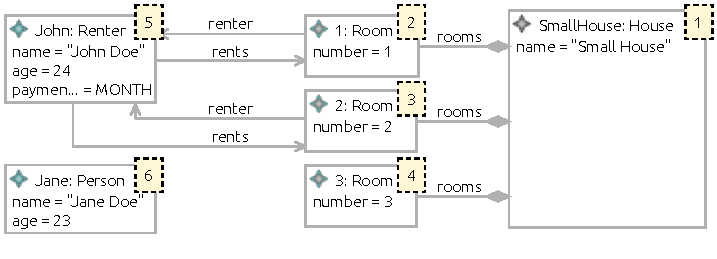
\includegraphics{images/03_formalisations/02_ecore_formalisation/properties/invalid_abstract.pdf}
    \caption{Model not satisfying the $\type{abstract}$ property.}
    \label{fig:formalisations:ecore_formalisation:instance_models:properties:abstract}
\end{figure}

\cref{fig:formalisations:ecore_formalisation:instance_models:instance_model_example} shows an example of an instance model that satisfies the $[ \type{abstract}, \type{Person} ]$ property, as no direct instantiations of the $\type{Person}$ class exist. On the other hand, \cref{fig:formalisations:ecore_formalisation:instance_models:properties:abstract} shows an instance model that does not satisfy the property, as the $\type{Person}$ class has been instantiated (by the object $\type{Jane}$).

\begin{figure}[p]
    \centering
    \begin{subfigure}{0.35\textwidth}
        \centering
        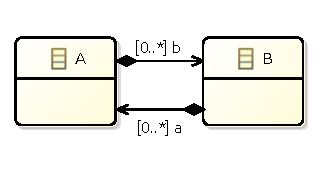
\includegraphics{images/03_formalisations/02_ecore_formalisation/properties/containment/type_model.pdf}
        \caption{Example type model with two containment relations}
        \label{fig:formalisations:ecore_formalisation:instance_models:properties:containment:type_model}
    \end{subfigure}
    \begin{subfigure}{0.3\textwidth}
        \centering
        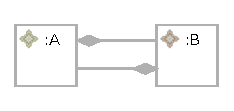
\includegraphics{images/03_formalisations/02_ecore_formalisation/properties/containment/invalid.pdf}
        \caption{Model not satisfying the containment property}
        \label{fig:formalisations:ecore_formalisation:instance_models:properties:containment:invalid}
    \end{subfigure}
    \begin{subfigure}{0.3\textwidth}
        \centering
        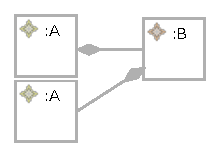
\includegraphics{images/03_formalisations/02_ecore_formalisation/properties/containment/valid.pdf}
        \caption{Model satisfying the containment property}
        \label{fig:formalisations:ecore_formalisation:instance_models:properties:containment:valid}
    \end{subfigure}
    \caption{Examples of the $\type{containment}$ property.}
    \label{fig:formalisations:ecore_formalisation:instance_models:properties:containment}
\end{figure}

\cref{fig:formalisations:ecore_formalisation:instance_models:properties:containment:type_model} shows a type model that defines two containment relations, in opposite direction. The instance model given in \cref{fig:formalisations:ecore_formalisation:instance_models:properties:containment:invalid} does not satisfy the satisfaction formula for the containment property, as there exists a cycle of containment relations. This is corrected in the instance model in \cref{fig:formalisations:ecore_formalisation:instance_models:properties:containment:valid}, where such a cycle does not exist (and each object is containment by at most one other object).

\begin{figure}[p]
    \centering
    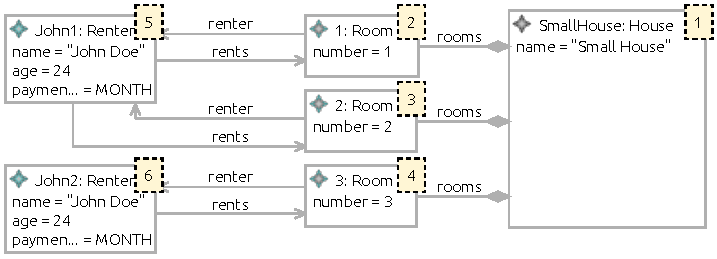
\includegraphics{images/03_formalisations/02_ecore_formalisation/properties/invalid_identity.pdf}
    \caption{Model not satisfying the $\type{identity}$ property.}
    \label{fig:formalisations:ecore_formalisation:instance_models:properties:identity}
\end{figure}

To illustrate the satisfaction of a $\textsf{identity}$ property, assume the type model in \cref{fig:formalisations:ecore_formalisation:type_models:type_model_example} specifies an identity property for the $\type{name}$ and $\type{age}$ attributes of the $\type{Renter}$ object. Formally, we define the following property:
\begin{equation*}
  \big[ \textsf{identity}, .\type{Renter}, \big\{ ( .\type{Person}, \type{name} ), ( .\type{Person}, \type{age} ) \big\} \big]  
\end{equation*}

The example in \cref{fig:formalisations:ecore_formalisation:instance_models:properties:identity} shows an instance model that does not satisfy the property, as the $\type{Renter}$ objects share the same values for the $\type{name}$ and $\type{age}$ attributes, but are still identified as different objects. In \cref{fig:formalisations:ecore_formalisation:instance_models:instance_model_example} the values of the $\type{name}$ and $\type{age}$ attributes are not the same, and thus the property would be satisfied.

\begin{figure}[p]
    \centering
    \begin{subfigure}{0.45\textwidth}
        \centering
        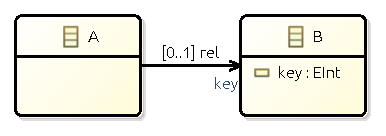
\includegraphics{images/03_formalisations/02_ecore_formalisation/properties/keyset/type_model.pdf}
        \caption{Example type model with relation $\type{rel}$ that has the keyset property defined on field $\type{key}$}
        \label{fig:formalisations:ecore_formalisation:instance_models:properties:keyset:type_model}
    \end{subfigure}
    \begin{subfigure}{0.25\textwidth}
        \centering
        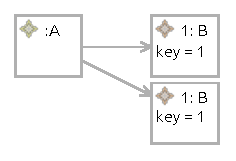
\includegraphics{images/03_formalisations/02_ecore_formalisation/properties/keyset/invalid.pdf}
        \caption{Model not satisfying the keyset property}
        \label{fig:formalisations:ecore_formalisation:instance_models:properties:keyset:invalid}
    \end{subfigure}
    \begin{subfigure}{0.25\textwidth}
        \centering
        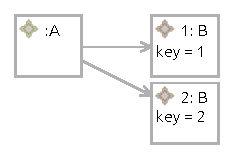
\includegraphics{images/03_formalisations/02_ecore_formalisation/properties/keyset/valid.pdf}
        \caption{Model satisfying the keyset property}
        \label{fig:formalisations:ecore_formalisation:instance_models:properties:keyset:valid}
    \end{subfigure}
    \caption{Examples of the $\type{keyset}$ property.}
    \label{fig:formalisations:ecore_formalisation:instance_models:properties:keyset}
\end{figure}

An example of the keyset property is shown in \cref{fig:formalisations:ecore_formalisation:instance_models:properties:keyset}. In \cref{fig:formalisations:ecore_formalisation:instance_models:properties:keyset:type_model}, we see the type model of this example. We assume there exists a class $\type{A}$ which can reference objects of class $\type{B}$ through relation $\type{rel}$. Furthermore, we assume that the $\type{key}$ field on class $\type{B}$ is used as key for the relation $\type{rel}$. In that case, \cref{fig:formalisations:ecore_formalisation:instance_models:properties:keyset:invalid} shows a violation of the $\type{keyset}$ property, because the 2 objects of type $\type{B}$ have the same value for $\type{key}$. In \cref{fig:formalisations:ecore_formalisation:instance_models:properties:keyset:valid}, the property is satisfied as both objects of type $\type{B}$ have a different value for $\type{key}$.

\begin{figure}[p]
    \centering
    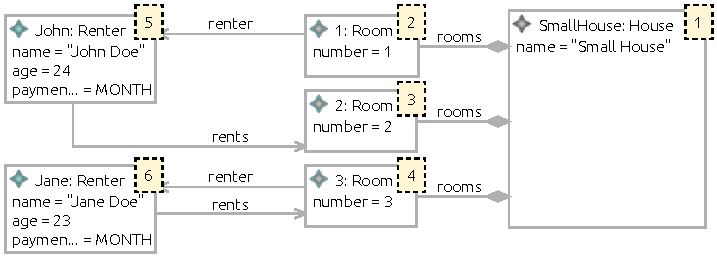
\includegraphics{images/03_formalisations/02_ecore_formalisation/properties/invalid_opposite.pdf}
    \caption{Model not satisfying the $\type{opposite}$ property.}
    \label{fig:formalisations:ecore_formalisation:instance_models:properties:opposite}
\end{figure}

In \cref{fig:formalisations:ecore_formalisation:instance_models:properties:opposite}, an example model is shown which does not satisfy the opposite property for the $\type{rents}$ and $\type{renter}$ relations. Although the number of relations is equal, they do not have the same source and target objects (in opposite direction). The example model in \cref{fig:formalisations:ecore_formalisation:instance_models:instance_model_example} does in fact satisfy the property.

With the previous definitions, it is now possible to define when an instance model itself is valid, given its type model.

\begin{defin}[Model validity]
\label{defin:formalisations:ecore_formalisation:instance_models:model_validity}
An instance model $Im$ is said to be valid with respect to type model $Tm$ if and only if
\begin{itemize}
    \item All values are correctly typed: $\forall ( ( obj, f\!ield ), val ) \in \mathrm{FieldValue}_{Im}\!: val:_{Im} \mathrm{type}_{Tm}(f\!ield)$.
    \item All container multiplicities are valid: $\forall fv \in \mathrm{FieldValue}_{Im}\!: \mathrm{validMul}_{Im}(f\!v)$.
    \item All properties are satisfied: $\forall p \in Prop_{Tm}\!: Im \models p$
    \item All default values have the correct type: $\forall c \in Constant_{Tm}\!: \mathrm{DefaultValue}_{Im}(c):_{Im} \mathrm{ConstType}_{Tm}(c)$.
    \item $Tm$ is consistent, as defined in \cref{defin:formalisations:ecore_formalisation:type_models:type_model_consistency}.
\end{itemize}

The validity of $Im$ with respect to $Tm$ is written as $Tm \vdash Im$.
\isabellelref{instance_model}{Ecore.Instance_Model}
\end{defin}